\chapter{Stellar flares}

\section{Study on the feasibility of stellar flare detection}

Before starting to adapt the algorithm for detecting solar flares to this scenario, a study was conducted parallel to its development, to see if the energy from flares originating in far-away stars could be detected using the already existing method, namely the GNSS Solar Flare Activity Indicator (GSFLAI) algorithms \cite{hernandez2012gnss}.

To study if this was feasible, the existing algorithm was executed with certain candidates of flares and GRBs to see if they could be detected.

The project supervisor, Manuel Hernández-Pajares, who as mentioned before has previously performed several studies on the subject, performed these tests with the GSFLAI algorithm. This algorithm takes into consideration the location of the source (the Sun) to see if there's a relation between an increase in the VTEC of the ionosphere and the solar-zenith angle to determine if this increase is caused by a solar flare \cite{hernandez2012gnss}. The aim was changing the location of the source (the Sun) to that of the star being studied to see if had any effect on the ionosphere.

However, because of its large execution time, the objective was to:

\begin{itemize}
	\item Find a database for possible candidates, several online archives with information about previously recorded Gamma Ray Bursts were considered.
	\item Select an appropriate source of this pool of candidates by writing a quick script that yielded an ordered list of the best candidates based on certain factors, instead of selecting a random source.
\end{itemize}

\subsection{Sources of data and possible candidates}

The three main databases we considered for the study were:

\begin{itemize}
	\item The GRB collection website of Jochen Greiner, scientist at the Max-Planck-Institute for extraterrestrial Physics (MPE) \cite{greinergrb},  which offers a collection of detected GRBs by different telescopes and observatories.
	\item The Magnetar Outburst Online Catalog (MOOC), developed by the Institute of Space Sciences (CSIC-IEEC, Barcelona) \cite{moocgrbs}. We also had the pleasure to meet one of the leaders of this project, Nanda Rea, and discuss
	\item The Neil Gehrels Swift Observatory website and archive by the National Aeronautics and Space Administration (NASA), Goddard Space Flight Center \cite{swiftnasa} which contains an archive of detected GRBs by the Swift observatory and is constantly updated.
\end{itemize}

Because of the layout of the website and how the data could be accessed, the option with which we started was the Swift Database, as the data could be visualized in an HTML table and was easily accessible.

\subsection{The Neil Gehrels Swift Observatory and its data}

The Swift Observatory is a NASA mission with international participation, designed to observe GRBs and their afterglows to study topics such as the origins of GRBs or what they can reveal about the early stages of the universe \cite{roming2005swift}. The observatory is equipped with three main instruments that work with each other to study GRBs \cite{gehrels2004swift} \cite{swiftnasa}:

\begin{itemize}
	\item The \textbf{Burst Alert Telescope (BAT)}, tasked with detecting the GRBs and computing their positions. This triggers the spacecraft to point the other telescopes to the burst so it can be studied in more detail. 
	\item The \textbf{X-ray Telescope (XRT)}, used for studying the X-ray radiation and taking images of the bursts which in turn help increase the accuracy of the location estimation.
	\item The \textbf{UV/Optical Telescope (UVOT)}, which serves a similar purpose to the XRT, but studies the ultraviolet band of the spectrum. 
\end{itemize}

For each detected GRB, the data obtained by the different telescopes is given. The parameters that are relevant to our study and determine the fitness of each of the candidates are:

\begin{itemize}
	\item The \textbf{name of the burst}, given by the date it was detected. For example, the GRB named 190220A was detected the 20th of February of 2019.
	\item The \textbf{Universal Time (UT)} of the detection, that is, hh:mm:ss of the day given by the name.
	\item The \textbf{fluence} detected by the BAT component, in units of keV.
	\item The \textbf{UVOT magnitude}, measured by the UV Telescope.
	\item The location that triggered the detection, given as \textbf{Right Ascension (Ra)} and \textbf{Declination (Dec)}.
\end{itemize}

\subsection{Objective function}

Our main goal in this section was to obtain a list of GRB candidates ordered from more to less probable to be detected by the algorithm based on their fitness. To obtain this score we had to define an objective function, taking into consideration two factors:

\begin{itemize}
	
	\item The \textbf{strength} of the burst, given by the UVOT magnitude. If this value was not available (as it was the case with many of the candidates) the BAT fluence was considered as its strength. This values were already given by the archive and no additional computations were required.
	
	\item The \textbf{angle between the burst and the Sun}, this was an important factor because bursts having an effect on the night hemisphere should be more noticeable than those hitting the day one, where the Sun has a bigger influence.
	
\end{itemize}

The final score is computed by adding the previous factors. While the angle ranged from 0 to 180, the strength had smaller values, giving more weight to the angle in the final score.

\paragraph{Computing the angle}

As mentioned before, the Swift archive gives us the Right Ascension (Ra) and Declination (Dec) where the source is thought to be located.

The location of the Sun, on the other hand, is unknown. But we do know the time when the burst was detected.

The supervisor, Manuel Hernández-Pajares, provided me with an algorithm which takes date (year, month, day and UT) and a planet of the Solar System (or the Sun, our case) as the input and returns its location in the celestial sphere, that is, its Ra and Dec. 

This algorithm belongs to the \textbf{Starlink Project} (Rutherford Appleton Laboratory), which provided open-source software like the one at hand to astronomical institutions. Although it was shut down in 2005, the code is still available and we could use it for our study \cite{starlinkproject}.

Knowing the location of the GRB and that of the Sun: the cosine of the angle between both can be computed and used as a parameter for the objective function.

\subsection{Obtaining the data}

Regarding the scrapping of the website to parse the data and obtain this ordered list, \textbf{Python} was chosen because the problem required a quick implementation, and Python’s libraries offered a great tool to develop a simple solution as quick as possible.

In the script, the website with the table of bursts (see figure x) is scrapped using Python’s \textbf{BeautifulSoup} library, which has an HTML and XML parser that allows us to easily select and obtain data from a given website.

Insertion sort was used so we could insert every considered GRB into a list of sorted candidates as we were traversing the table. 

The best 5 candidates of the resulting sorted table\footnote{until the moment of these tests}, are shown here:

\begin{table}[h!]
	\centering
	\def\arraystretch{1.2}
	\begin{tabular}{|c c c c c c c c|} 
		\hline
		Name & Ra & Dec & UVOT & BAT & Date & Angle & Score \\
		\hline\hline
		190202A & 166.506 & 9.393 & V=17.94 & 60 & 2019.02.02 & 148.79 & 166.69 \\
		\hline
		190129B & 117.285 & 1.257 & n/a & n/a & 2019.01.29 & 158.11 & 158.11 \\
		\hline
		181228A & 49.831 & 13.212 & V>19.1 & 100 & 2018.12.28 & 134.41 & 153.41 \\
		\hline
		181010A & 52.574 & -23.023 & V>19.4 & 6.9 & 2018.10.10 & 133.22 & 152.22 \\
		\hline
		190219A & 189.686 & 76.606 & n/a & 39 & 2019.02.19 & 111.74 & 150.74 \\
		\hline
	\end{tabular}
	\caption{Best results from the Swift GRB database}
\end{table}

Sadly, none of the GRBs provided good results, an example of the result of the execution of the GSFLAI algorithm is shown in figure \ref{fig:gsflai}

\begin{figure}[!htb]
	\begin{centering}
		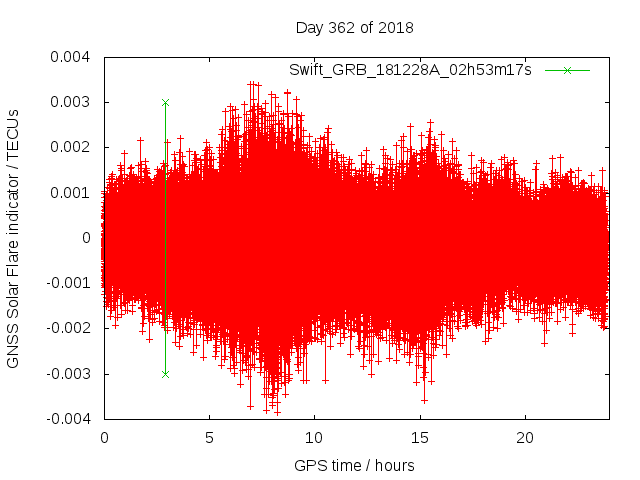
\includegraphics[width=0.5\linewidth]{images/swift/gsflai.png}
		\caption{Comparison of the real error (purple) and the estimated Least Squares error (green)}
		\label{fig:gsflai}
	\end{centering}
\end{figure}

As we can see, although a small peak can be seen at the moment of the flare...
TODO: completar esto

\section{Testing the BGSEES algorithm}

As we have seen detecting stellar flares is a really challenging task. Even when knowing the location of the star. (hacer referencia al capitulo de swift?) The aim of the project was to provide algorithms to detect Solar flares without knowing the location of the Sun to try this method  to do so with this method. 


Only two, they are harder to detect
More challenging

and flares from far-away stars. Because the day hemisphere has to be discarded in order to study far-away stars (because of the Sun's effect on the ionosphere), the first section will study examples of flares originating from the Sun and the second those from outside the Solar System. -> En este capitulo al final solo sol, estrellas en el siguiente

\subsection{Discarding the day hemisphere}

One of the first things that needed to be implemented in order to study stellar flares was a way to avoid the interferences of the Sun. Because the Sun would have a greater effect on the Earth's ionosphere, the day hemisphere is discarded.

This leaves the algorithm with only half the data and potential flares could be missed if they were affecting the day hemisphere.

This is done by simply taking the IPP's and Sun's right ascension and declination from the ti file and computing the cosine of their angle as has been done in previous chapters, using equations \ref{eq:3}, \ref{eq:4} and \ref{eq:5}.

If we want to discard the day hemisphere, then the IPP has to be ignored if the cosine of the angle, which has a range of [-1,1], is smaller than -0.1 (the point at which a linear correlation between the variables can be observed, as seen in chapter 4 (figure \ref{fig:results}).

The following is the AWK script that performs this check for every IPP if we indicate the algorithm that it has to discard the hemisphere:

\begin{minipage}{\linewidth}
	\begin{lstlisting}[language=awk, caption=Discarding the day hemisphere]
	function checkValidIPP(raSun, decSun, raIPP, decIPP) {
		return unitVectorsCosine(raSun, decSun, raIPP, decIPP) >= -0.1
	}
	
	function unitVectorsCosine(raSource, decSource, raIPP, decIPP) {
		return (sin(decIPP)*sin(decSource) + cos(decIPP)*cos(decSource)*cos(raIPP - raSource));
	}
\end{lstlisting}
\end{minipage}

With this change in the algorithm, it should be ready to try to detect stellar flares, rather than flares from the Sun. The following are some cases of strong stellar flares detected by dedicated telescopes that have been presented in research papers, using the information of them and with the help of the authors in some cases, the algorithm is tested to see if it can work with stellar flares or these are too weak to be detected without a dedicated telescope. 

\subsection{Proxima Centauri}

The first studied flare is presented in the paper \textit{"The first naked-eye superflare detected from Proxima Centauri"} (Howard, Ward S., et al.) \cite{howard2018first}, which, as the title of the paper suggests, was a flare so powerful it could even be seen with the naked eye. However, the flare could not be detected by pointing directly at it (knowing the location). This star is located in the Centaurus constellation, 4.22 light-years away

The flare was detected the 18th of March of 2016, with the flare peaking at 8:32 UT. Having the ti file from this day in particular, 2016.078, we filtered the time range to obtain one hour surrounding that specific moment. Because this was a more challenging scenario, instead of finding the moment of the peak and only focusing on that time, the algorithm iterates over all epochs to see if any of them provided good results.

Taking into consideration that Proxima Centauri has a right ascension of $217.4294^{\circ}$ and a declination of $-62.67948^{\circ}$ \cite{proximawiki}, the algorithm was executed using only the night hemisphere to try to detect this flare, using this location to calculate the error of the estimation.

ITERATE OVER ALL EPOCHS

\subsection{NGTS J121939.5-355557}

Another studied stellar flare is presented in the paper \textit{"Detection of a giant flare displaying quasi-periodic pulsations from a pre-main-sequence M star by the Next Generation Transit Survey"} (Jackman, James AG, et al.) \cite{jackman2018detection}. 

Although the date was specified in the paper (2016.032), the specific moment of the flare was not indicated. We got in touch with the authors of the paper, who kindly provided us information about the moment of the flare. The event was detected only at the moment of the peak (04:00 UT), so the start and end of the flare were unknown. Because of this, we worked with one hour of data surrounding the peak.


Because we obtained some relatively good results with some cases using this epoch, we decided to study this one more in detail.


hablar de que aqui se me ocurrio el tema de 2 epocas, 0.2 en el coseno, etc

ITERATE OVER ALL EPOCHS



